\beginsong{Was helfen mir tausend Dukaten}[
    wuw={aus Schlesien nach Hoffmann/Richter}, 
    bo={362}, 
    siru={251},
]

\beginverse
\endverse
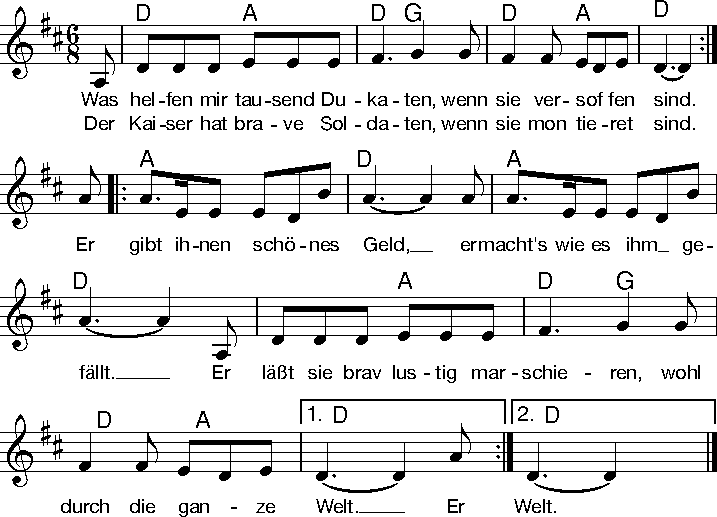
\includegraphics[draft=false, width=1\textwidth]{Noten/Lied092.pdf}

\beginverse
Ei, \[D]Bauer, das \[A]tu ich dir \[D]sa\[G]gen: Wenn \[D]mein Quar\[A]tier ist \[D]aus,
wenn \[D]die Trom\[A]peter \[D]bla\[G]sen, so \[D]wecke \[A]mich bald \[D]auf
\lrep und \[A]sattle mir mein \[D]Pferd und \[A]rüste mir mein \[D]Schwert,
den Mantel, den \[A]tu mir drauf \[D]bin\[G]den, dass \[D]ich bald \[A]fertig \[D]werd'. \rrep
\endverse
\beginverse

Der ^Tag fing ^an zu ^bre^chen, der ^Wirt stand ^in der ^Tür,
tat ^zu den ^Reitern ^spre^chen: "Trom^peter ^sind schon ^hier.
\lrep Sie ^blasen alle frisch ^auf, ihr ^Herren Soldaten steht ^auf!
Das Pferd ist ^schon ge^sat^telt, der ^Mantel ge^bunden da^rauf. \rrep
\endverse
\beginverse

''Ei, ^Rösslein, das ^tu ich dir ^sa^gen: den ^Sporen ^geb' ich ^dir,
du ^musst mich ^heute noch ^tra^gen vor ^meiner Herz^liebsten ^Tür'',
\lrep wohl ^vor das hohe ^Haus, da ^schaut das Mädel he^raus
mit ihren ^schwarz-braunen Ä^uge^lein, zum ^Fenster ^schaut sie he^raus. \rrep
\endverse

\endsong

\beginscripture{}
Dukaten = Goldmünzen
\endscripture
